\section{Approach}
In this section, we present our implementation for injecting faults, as well as analysis for predicting program outcome and fault types.

\subsection{Pipeline}
Figure~\ref{fig:pipeline} shows the general pipeline of our proposed system. For any target application, it is first modified to contain at least one all to initialize fault injection. Then it is compiled in the architecture X86 or ALPHA where GemFI support with the specific libraries. In this work, we choose ALPHA as our test architecture as it is lightweight and have full supports by the fault injector. Afterwards, the generated binary should be moved to the disk image serving as the virtual disk of GemFI. The specific faults are provided by the user in a file at command line. Each line of the input file specifies the attributes of a single fault. We will talk in detail about the fault injection in Section \ref{section:FI}. 

GemFi simulator simulates the execution of the 

\begin{figure*}[t]
\begin{center}
   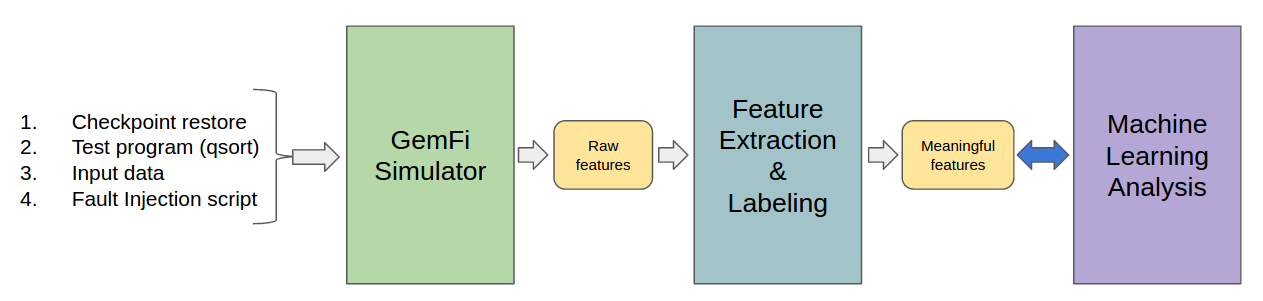
\includegraphics[width=0.95\linewidth]{./figures/pipeline.png}
\end{center}
   \caption{}
\label{fig:pipeline}
\end{figure*}



\subsection{Fault Injection}\label{section:FI}
GemFI \cite{parasyris2014gemfi} supports two kind of architectures: ALPHA and X86. In our project, we choose ALPHA as our test architecture. In order to inject faults into the test program, it needs to be modified to initialize the fault injection. The target application is cross-compiled by the alpha gnu toolchain and linked with FI libraries. Afterwards, the generated binary should be moved to the disk image serving as the virtual disk of GemFI. The specific faults are provided by the user in a file at command line. Each line of the input file specifies the attributes of a single fault. Faults are characterized by four attributes: Location, Thread, Time and Behavior. 

An example below shows the a sample input of faults. 
\begin{lstlisting}[language=bash]
RegisterInjectedFault Inst:2457 Flip:21 Threadid:0 system.cpu1 occ:1 int 1
\end{lstlisting}

This example describes a fault that injects into the $21st$ bit of the register R1 of the CPU, when the application fetches $2457th$ instruction after the initiation of fault injection. For our current tests, we just generate faults by randomly sampling from the number of instructions of the test program, the components of ALPHA and the operations needed. However, this method couldn't cause the program to generate false results some time as different programs make use of different components at different time. So we will explore the running characteristics of each test program and generate faults from a finer and smaller space. 

\begin{figure}[t]
\begin{center}
   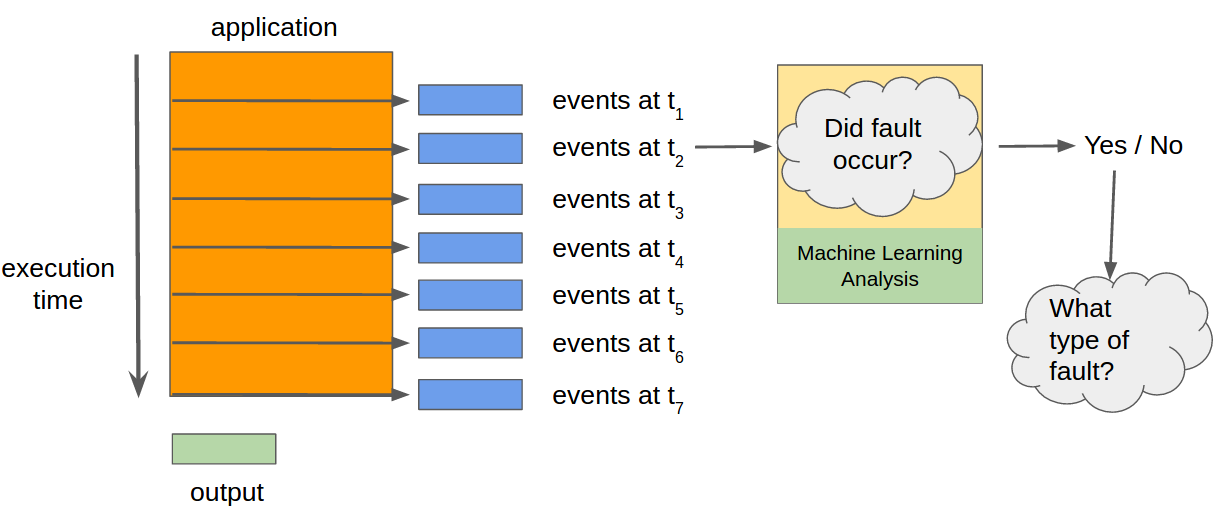
\includegraphics[width=0.95\linewidth]{./figures/teaser.png}
\end{center}
   \caption{Motivation to extract meaningful features}
\label{fig:teaser}
\end{figure}

\subsection{Feature Extraction}
We extract all the common features from the \emph{stats} files generated by GemFI. Since some fault injected program will generate fewer features than non-fault injected program, we only choose those the features appeared in both programs.
\begin{figure*}[t]
\begin{center}
   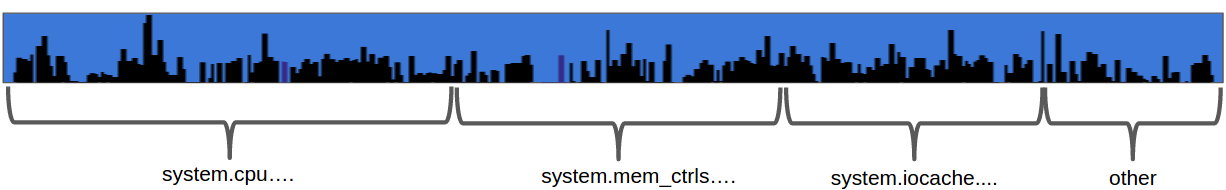
\includegraphics[width=0.95\linewidth]{./figures/feat_dist.png}
\end{center}
   \caption{}
\label{fig:feat-dist}
\end{figure*}


\subsection{Machine Learning Method}\label{section:ML}
We use the random forest algorithm to predict program outcome and fault type. A random forest is essentially an ensemble of single decision trees \cite{breiman2001random}. It captures different characteristics of the data, with each decision tree representing a model. One particular attractive aspect of random forest is that it allows us to analyze the importance of different features according to the information gain of each feature dimensions. We can use the information gain to rank the importance of each feature and therefore determine which features can be pruned.

%\begin{figure}[t]
%\begin{center}
%   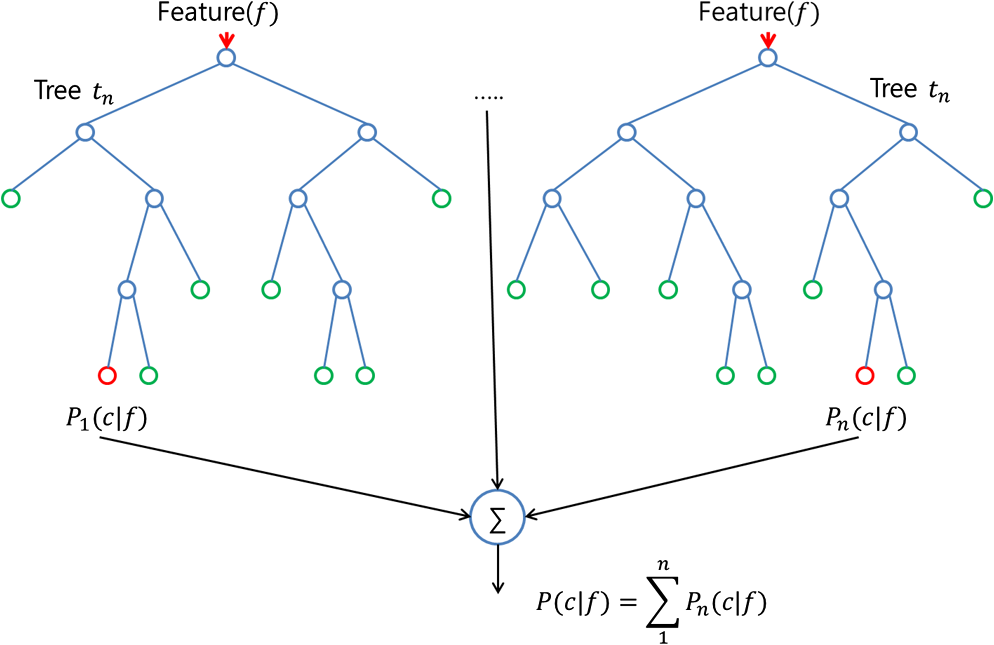
\includegraphics[width=0.95\linewidth]{./figures/rf.png}
%\end{center}
%   \caption{\footnotesize Random forests}
%\label{fig:rf}
%\end{figure}


%\begin{figure}[t]
%\begin{center}
%   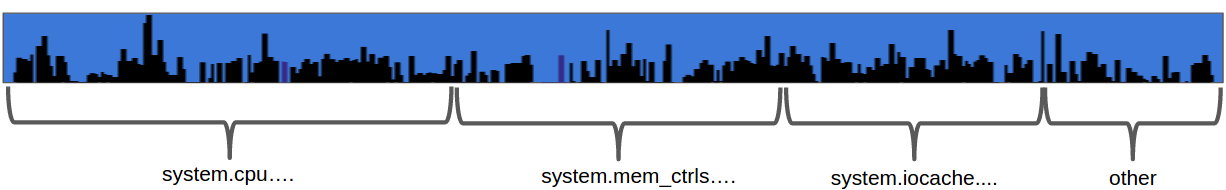
\includegraphics[width=0.95\linewidth]{./figures/feat_dist.png}
%\end{center}
%   \caption{\footnotesize Features in different components of the microachitecture.}
%   \vspace{-0.4cm}
%\label{fig:feat-dist}
%\end{figure}

%Figure~\ref{fig:feat-dist} shows features in different components of the microarchitecture.

We randomly select $60\%$ of instances for training and $40\%$ of instances for testing. Our dataset consists of $98,000$ data instance.
